\documentclass[aspectratio=169,11pt]{beamer}
\usetheme{Madrid}
\usecolortheme{default}
\usepackage{amsmath,amssymb,graphicx,booktabs}
\usepackage{hyperref}
\usepackage{tikz}
\usetikzlibrary{arrows.meta, positioning, fit, backgrounds, shapes.geometric, calc}
\tikzset{
  flowarr/.style={-{Stealth[length=2.2mm]}, thick, draw=gray!65},
  stepnum/.style={circle, draw=structure.fg!40, fill=white,
                  font=\bfseries\footnotesize, inner sep=0pt, minimum size=0.52cm},
  databox/.style={draw=green!50!black, rounded corners=4pt, align=center,
                  font=\small, text width=5.6cm, minimum height=0.72cm, fill=green!8},
  modelbox/.style={draw=blue!50!black, rounded corners=4pt, align=center,
                   font=\small, text width=5.6cm, minimum height=0.72cm, fill=blue!8},
  searchbox/.style={draw=orange!70!black, rounded corners=4pt, align=center,
                    font=\small, text width=5.6cm, minimum height=0.72cm, fill=orange!10},
  checkbox/.style={draw=violet!60!black, rounded corners=4pt, align=center,
                   font=\small, text width=5.6cm, minimum height=0.72cm, fill=violet!8},
  decision/.style={draw=red!60!black, diamond, aspect=2.2, align=center,
                   font=\scriptsize, inner sep=0.5pt, fill=red!6},
  flowscale/.style={transform shape, scale=0.78},
  vflowbox/.style={rounded corners=4pt, align=center, font=\footnotesize,
                   text width=5.2cm, minimum height=0.9cm, inner sep=4pt},
  vflowarr/.style={-{Stealth[length=2mm]}, thick, draw=gray!55},
  vflowkey/.style={rounded corners=4pt, align=center, font=\scriptsize\bfseries,
                   text width=5.8cm, minimum height=0.88cm, inner sep=5pt,
                   draw=orange!85!black, fill=orange!22, line width=1.9pt},
}

\title{Aligning model behavior with domain expectations via interventional audits}
\author{Jonas Wolber \& Moein Samadi}
\date{\today}

\newcommand{\img}[2]{\includegraphics[width=#1\textwidth]{images/#2}}

\begin{document}

% ------------------------------------------------------------------
\begin{frame}
  \titlepage
\end{frame}

% ------------------------------------------------------------------
\begin{frame}{Case study: Ohio T1DM dataset}
  \begin{columns}[T]
    \column{0.40\textwidth}
    \begin{itemize}
      \item Features: insulin impact curve, carbs impact curve, Physical activity sensors, glucose dynamics
      \item Target: future glucose change at 30 minutes
      \item Models may mislearn insulin effects when \textbf{meals and boluses co-occur} --- carbs and insulin features rise together, confounding the learned insulin--glucose association.
    \end{itemize}
    \column{0.58\textwidth}
    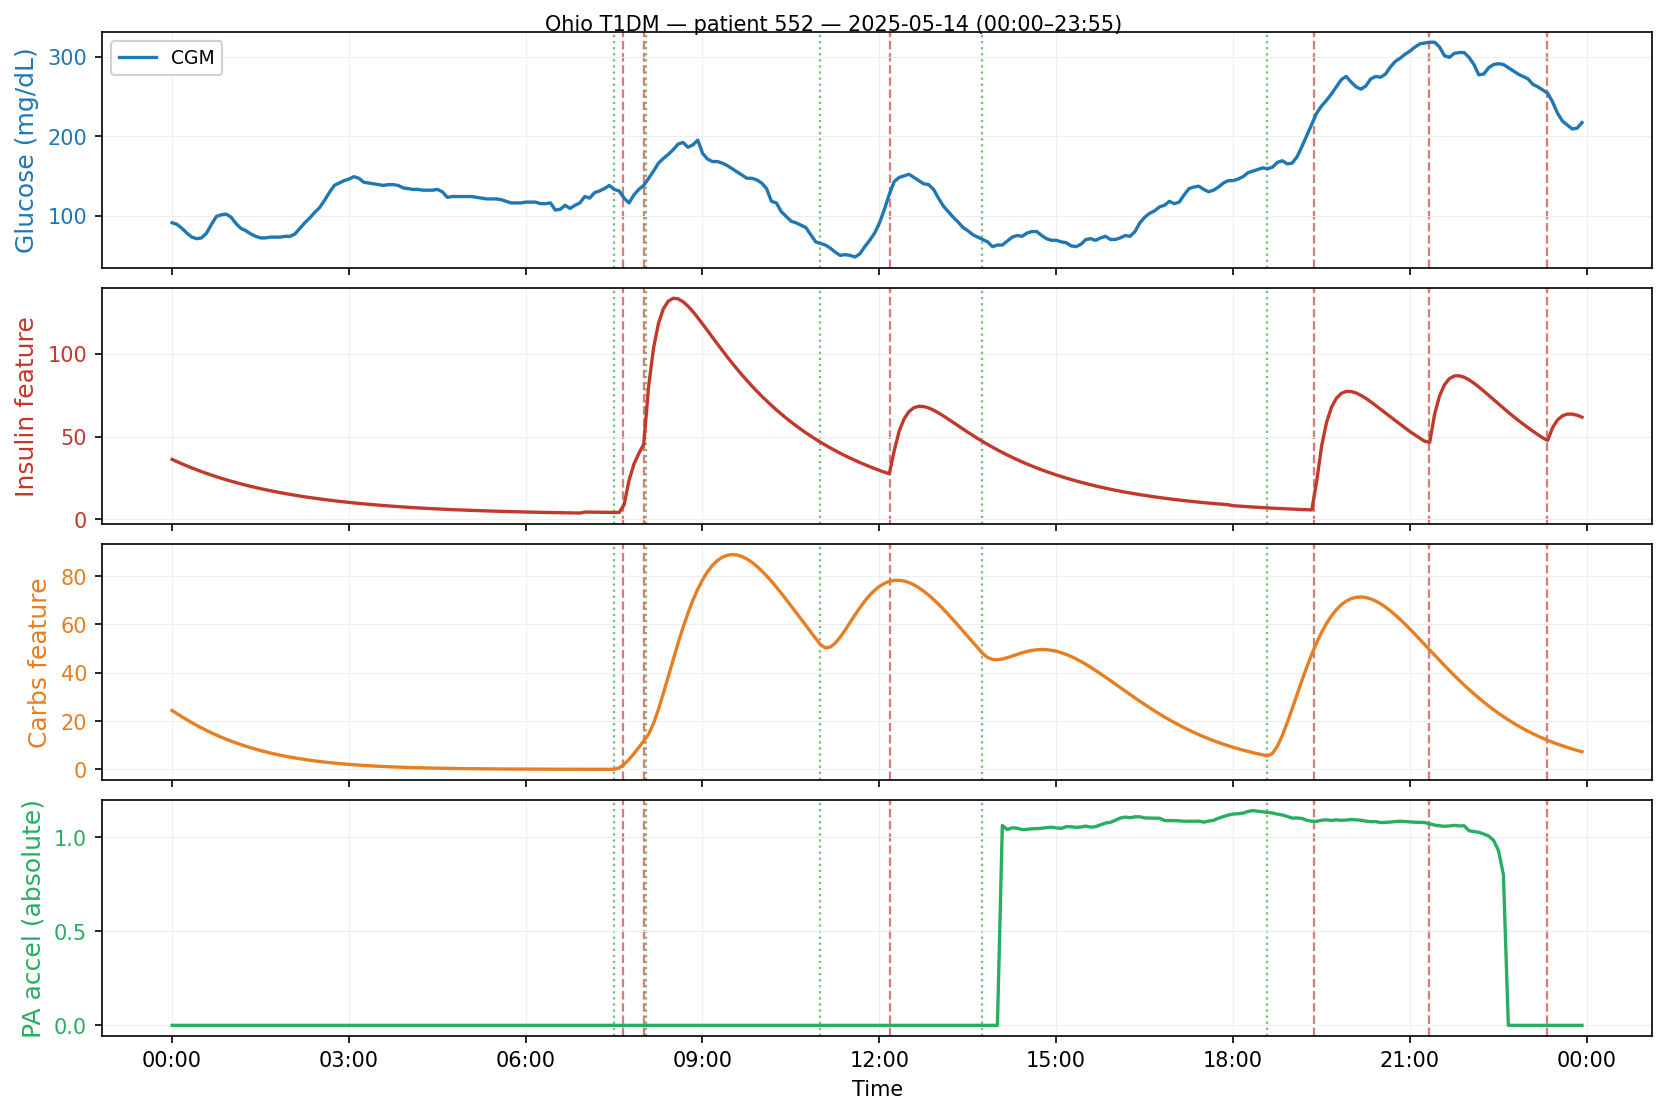
\includegraphics[width=\linewidth,height=0.72\textheight,keepaspectratio]{images/preprocess_example_insulin_glucose.png}
  \end{columns}
\end{frame}

% ------------------------------------------------------------------
\begin{frame}{The problem: accurate predictions but wrong feature attributions}
  \begin{columns}[T]
    \column{0.44\textwidth}
    \begin{itemize}
      \item Predictive models can achieve \textbf{low RMSE} yet encode \textbf{wrong or inconsistent feature attributions} contradictory to domain expectations.
      \item \textbf{Baseline SHAP} values can suggest but not quantify these inconsistencies.
      \item Clinical expectation: more insulin should \textbf{lower} future glucose.
      \item SHAP alone does not test that counterfactual; we need an \textbf{interventional audit}
    \end{itemize}
    \column{0.54\textwidth}
    \img{1.0}{01_shap_baseline_problem.png}
    \vspace{0.2em}
    \centering\small\textbf{SHAP beeswarm} --- Ohio T1DM patient 588, baseline LightGBM
  \end{columns}
\end{frame}

% ------------------------------------------------------------------
\begin{frame}{Interventional response curves (Partial dependence plots)}
  \small
  \begin{columns}[T]
    \column{0.5\textwidth}
    \begin{itemize}
      \item \textbf{Interventional response curve (IRC):} For each level $g$ of a feature $X$, we perform an intervention $\mathrm{do}(x = g)$ (holding all other features fixed) and compute the mean model prediction $\hat{y}$ for the target variable.
      \item Clinical expectations: monotonic relationships between insulin, carbs, and activity and the target variable (future blood glucose).insulin $\searrow$, carbs $\nearrow$, activity $\searrow$.
      \item Actual curves: we see violations of these expectations in the curves as indicated by the orange lines.
    \end{itemize}
    \column{0.5\textwidth}
    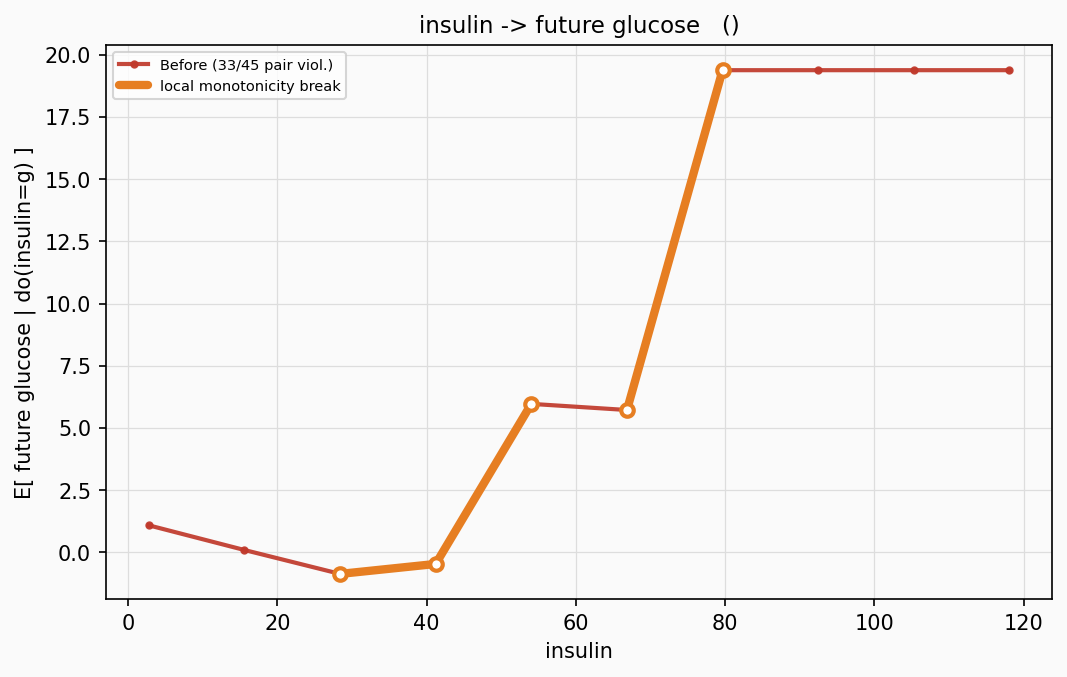
\includegraphics[width=\linewidth,height=0.26\textheight,keepaspectratio]{images/01_insulin_interventional_response_curve.png}
    {\centering\tiny Insulin --- p.\,588; $\searrow$ expected (33/45)\par}
    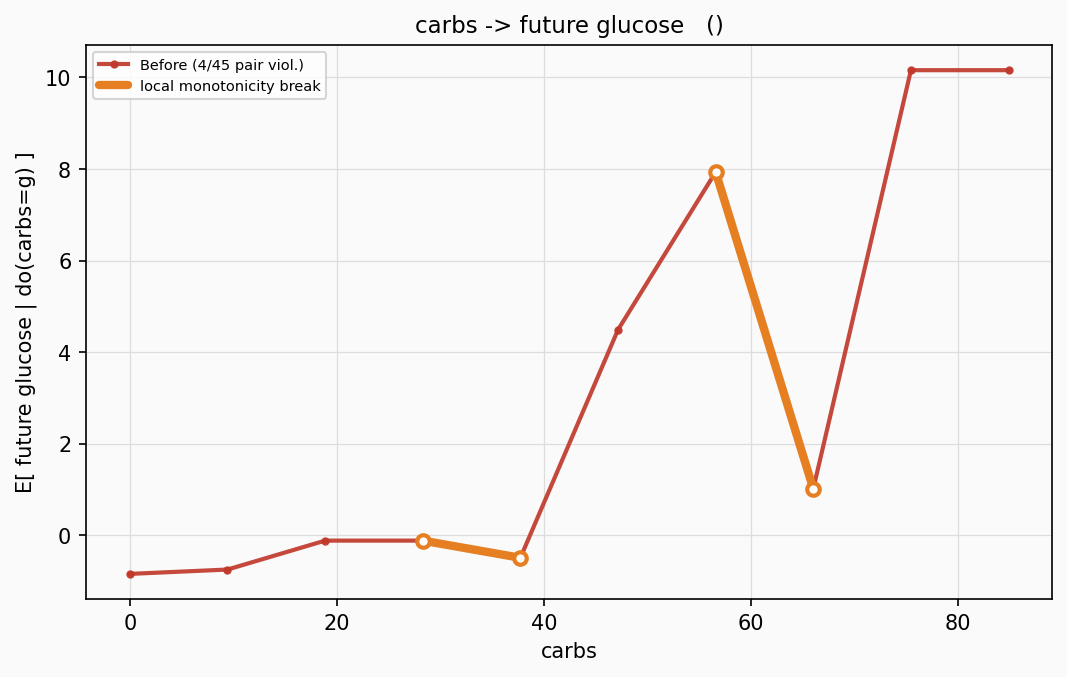
\includegraphics[width=\linewidth,height=0.26\textheight,keepaspectratio]{images/01_carbs_interventional_response_curve.png}
    {\centering\tiny Carbs --- p.\,591; $\nearrow$ expected (4/45)\par}
    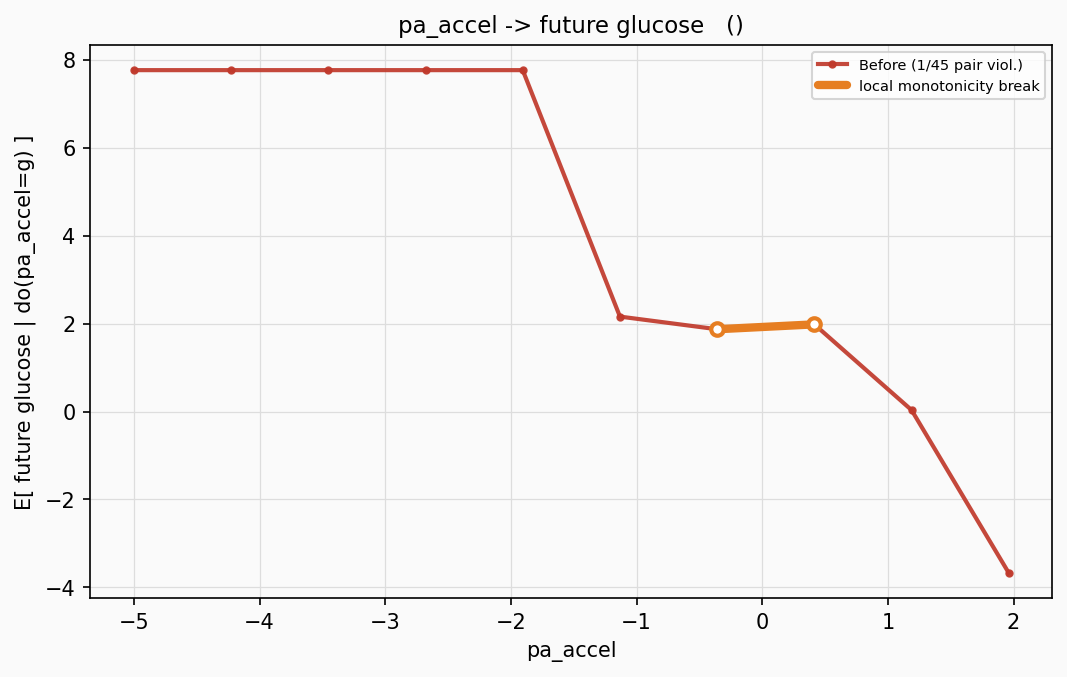
\includegraphics[width=\linewidth,height=0.26\textheight,keepaspectratio]{images/01_pa_accel_interventional_response_curve.png}
    {\centering\tiny Accel.\ --- p.\,567; $\searrow$ expected (1/45)\par}
  \end{columns}
\end{frame}

% ------------------------------------------------------------------
\begin{frame}{What can we derive from Interventional response curves?}
  \begin{columns}[T]
    \column{0.3\textwidth}
    \small
    \begin{itemize}
      \item \textbf{Direct feature contributions (upper panels) and feature interactions (lower panels)}
      \item \textbf{Function characteristics}: Monotonicity (left panels), specific functions, e.g. sigmoid or sinusoidal (middle panels), causal independence (right panels)
    \end{itemize}
    \column{0.7\textwidth}
    \centering
    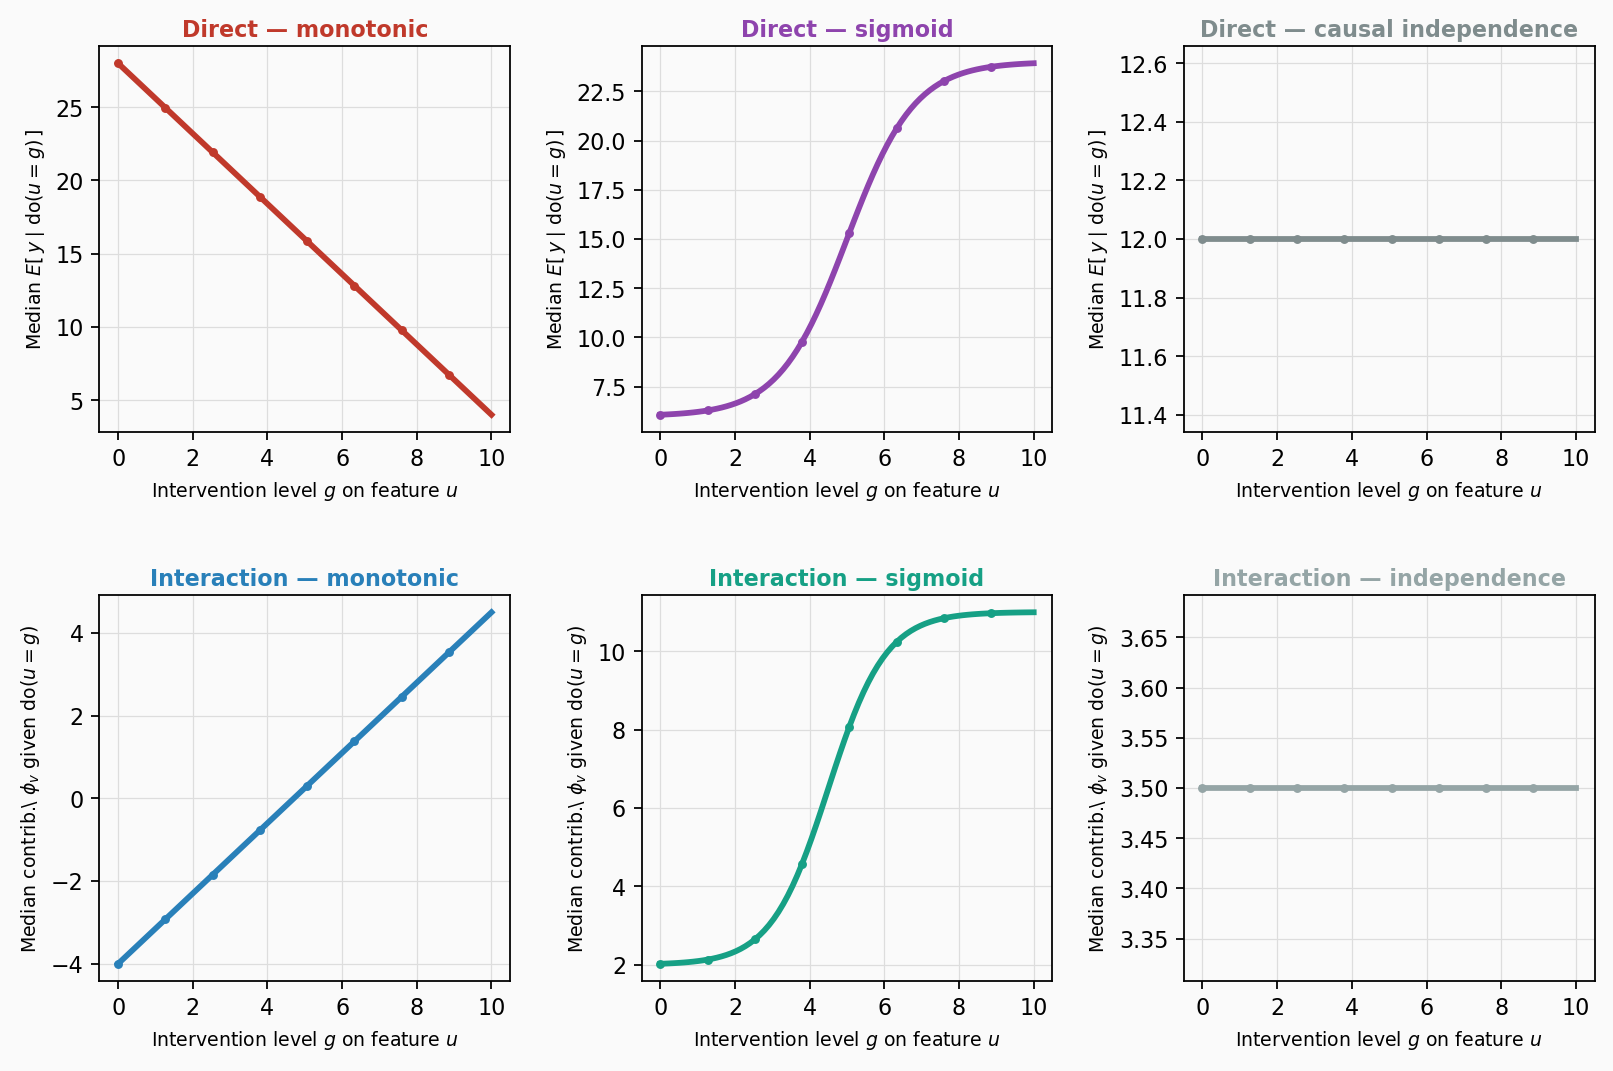
\includegraphics[width=0.9\linewidth]{images/irc_six_relationship_types.png}
  \end{columns}
\end{frame}

% ------------------------------------------------------------------
\begin{frame}{Evaluating the alignment of the interventional response curves with expected behavior}
  \begin{columns}[T]
    \column{0.34\textwidth}
    \small
    \textbf{Violations of Monotonicity}

    \vspace{0.5em}
    \textbf{Goodness of fit of the interventional response curve to the function modeling expected behavior}
    \vspace{0.5em}

    We can define expected behavior with a Structural Causal Model (SCM) with additional instructions on edge characteristics.
    \column{0.66\textwidth}
    \centering
    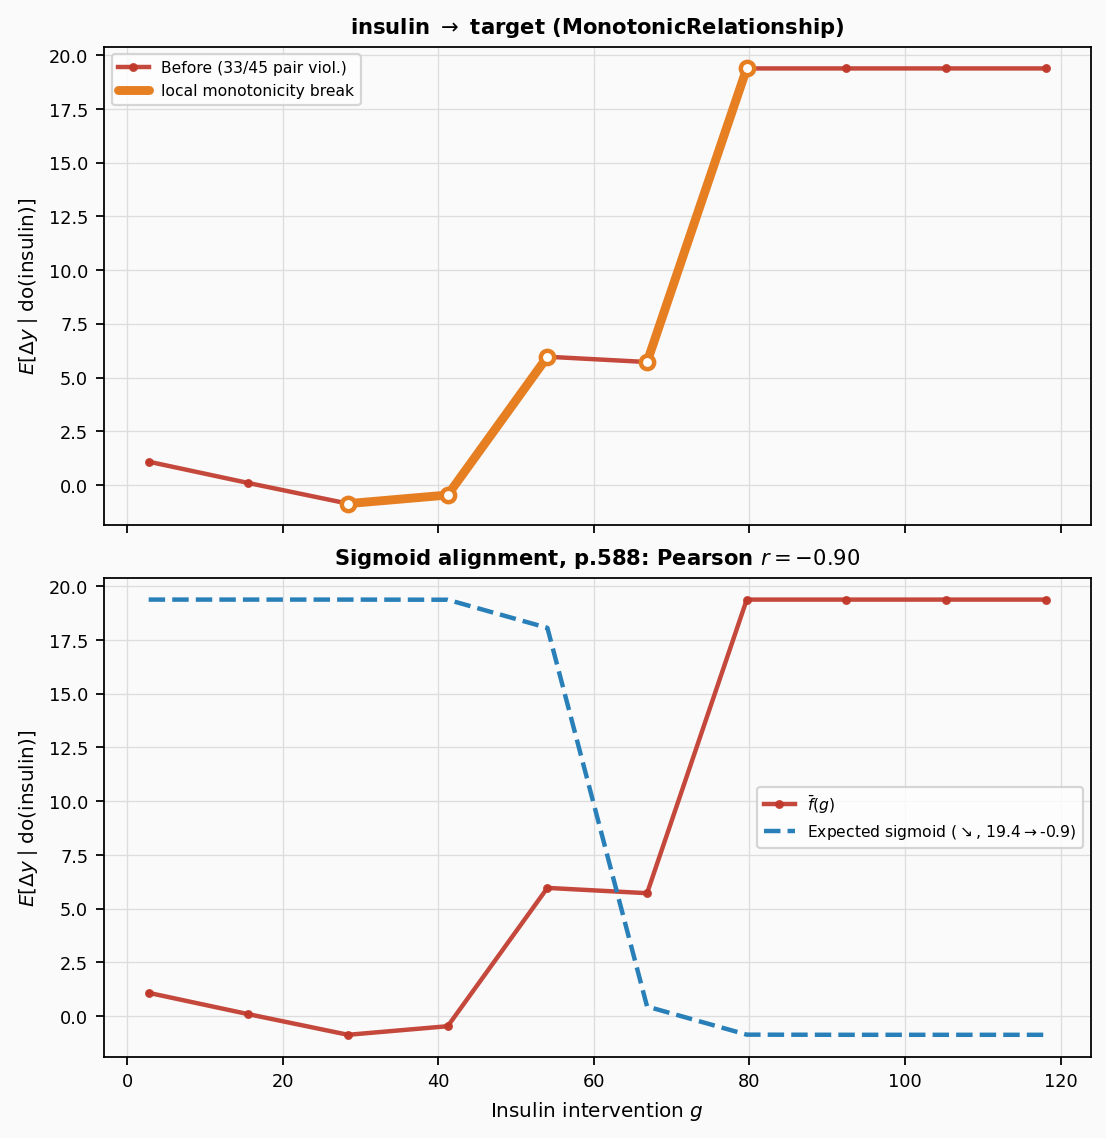
\includegraphics[width=\linewidth,height=0.78\textheight,keepaspectratio]{images/irc_alignment_examples.png}
    {\centering\tiny Baseline insulin IRC, p.\,588 --- model learned $\nearrow$ (wrong sign)\par}
  \end{columns}
\end{frame}

% ------------------------------------------------------------------
\begin{frame}{Approaches for aligning model behavior with domain expectations}
  \scriptsize
  \begin{tabular}{@{}p{0.58\textwidth}p{0.40\textwidth}@{}}
    \toprule
    \textbf{Approach} & \textbf{Studies} \\
    \midrule
    \textbf{Model learning:} encode SCM monotonicity signs as constraints during training (monotone tree splits, constrained optimization, or penalty terms).
    & \textbf{Wolber (2025)}; Koklev (2025); Xie \& Tummala (2025); Borghesi et al.\ (2020) \\[0.4em]
    \textbf{Model architecture:} bake domain structure into the network---e.g.\ physiological LSTM with fixed insulin/CHO preprocessing layers that separate time-action profiles before sequence modeling.
    & Prendin et al.\ (2023) \\[0.4em]
    \textbf{Preprocessing:} residualize insulin against glucose-context features so bolus signal is orthogonal to confounding CGM dynamics before any learner.
    & Akinwumi et al.\ (2026) \\[0.4em]
    \textbf{Feature engineering:} add explicit insulin--context and carbs--context interaction terms to expose meal--bolus co-occurrence in the input space.
    & Butt et al.\ (2023); Beauchamp et al.\ (2021) \\[0.4em]
    \textbf{Synthetic augmentation:} generate SCM-aligned synthetic rows.
    & Noguer et al.\ (2022); Prendin \& Facchinetti (2025); Kalita et al.\ (2024) \\[0.4em]
    \textbf{Latent confounder:} impute latent confounder feature(s) from feature interactions
    & Sun et al.\ (2020--2023); Bing et al.\ (2022); Prendin et al.\ (2023) \\
    \bottomrule
  \end{tabular}
\end{frame}

% ------------------------------------------------------------------
\begin{frame}{What our approach aims to do differently}
  \small
  \textbf{IRAlign} =  align tabular models with domain rules using interventional response curves.
  \begin{columns}[T]
    \column{0.48\textwidth}
    \begin{itemize}
      \item \textbf{No accuracy compromise} --- RMSE/feasibility trade-off (e.g. on Pareto front).
      \item \textbf{Model-agnostic} --- wraps any tabular model.
      \item \textbf{Fast IRC scoring} 
      \item \textbf{Flexible rules} --- monotonic, sigmoid, flat, etc; implementable not only for Diabetes modeling
    \end{itemize}
    \column{0.48\textwidth}
    \begin{block}{Under investigation}
      We currently investigate two approaches: Synthetic augmentation vs.\ latent confounder imputation.
    \end{block}
  \end{columns}
\end{frame}

% ------------------------------------------------------------------
\begin{frame}{Approach A: Synthetic data augmentation}
  \small
  \begin{columns}[T]
    \column{0.40\textwidth}
    \begin{alertblock}{Idea}
      \textbf{Add synthetic training rows} the patient never logged --- e.g. insulin boluses in the absence of meals. A diabetic patient would rarely do this. However, these datapoints are needed to learn correct insulin behavior.
    \end{alertblock}

    \column{0.58\textwidth}
    \centering
    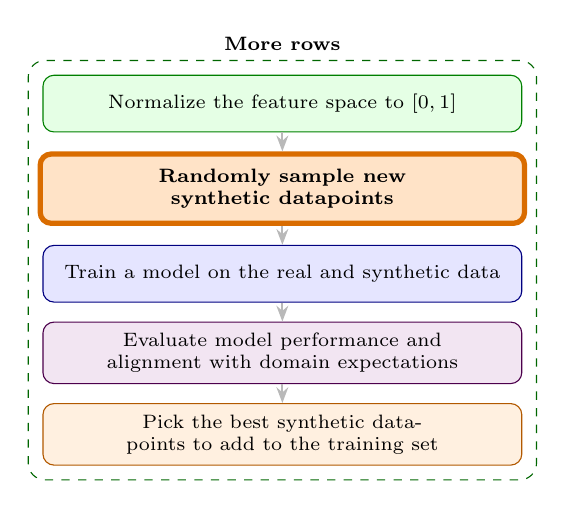
\begin{tikzpicture}[
      node distance=0.24cm,
      vflowbox/.append style={text width=5.8cm, minimum height=0.72cm, font=\scriptsize},
      databox/.append style={vflowbox, draw=green!50!black, fill=green!10},
      searchbox/.append style={vflowbox, draw=orange!70!black, fill=orange!12},
      modelbox/.append style={vflowbox, draw=blue!50!black, fill=blue!10},
      checkbox/.append style={vflowbox, draw=violet!60!black, fill=violet!10},
    ]
      \node[databox] (s1) {Normalize the feature space to $[0,1]$};
      \node[vflowkey, below=of s1] (s2) {Randomly sample new synthetic datapoints};
      \node[modelbox, below=of s2] (s3) {Train a model on the real and synthetic data};
      \node[checkbox, below=of s3] (s4) {Evaluate model performance and alignment with domain expectations};
      \node[searchbox, below=of s4] (s5) {Pick the best synthetic datapoints to add to the training set};

      \foreach \a/\b in {s1/s2, s2/s3, s3/s4, s4/s5} {
        \draw[vflowarr] (\a) -- (\b);
      }

      \node[draw=green!40!black, dashed, rounded corners=6pt, fit=(s1)(s5),
            inner sep=0.18cm, label={[font=\scriptsize\bfseries]above:More rows}] {};
    \end{tikzpicture}
  \end{columns}
\end{frame}

% ------------------------------------------------------------------
\begin{frame}{Approach B: Latent confounder imputation}
  \small
  \begin{columns}[T]
    \column{0.40\textwidth}
    \begin{alertblock}{Idea}
      \textbf{Add a latent confounder feature} --- a new column from a formula over SHAP interaction values --- to represent unobserved drivers the sensors never record: e.g.\ meal overestimation, circadian rhythm, absorption variability, or combined interaction effects that distort the insulin--glucose link.
    \end{alertblock}

    \column{0.58\textwidth}
    \centering
    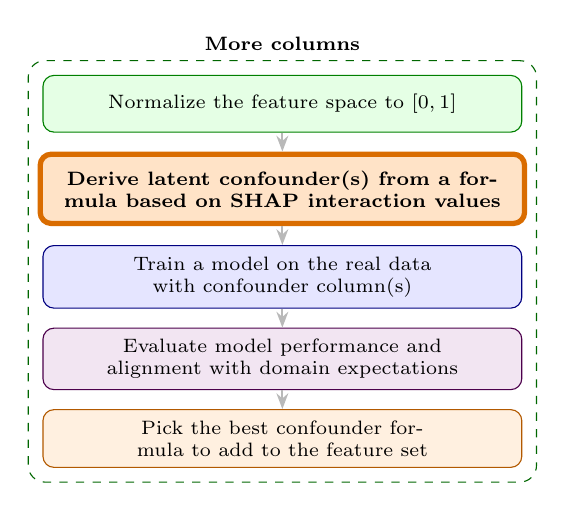
\begin{tikzpicture}[
      node distance=0.24cm,
      vflowbox/.append style={text width=5.8cm, minimum height=0.72cm, font=\scriptsize},
      databox/.append style={vflowbox, draw=green!50!black, fill=green!10},
      searchbox/.append style={vflowbox, draw=orange!70!black, fill=orange!12},
      modelbox/.append style={vflowbox, draw=blue!50!black, fill=blue!10},
      checkbox/.append style={vflowbox, draw=violet!60!black, fill=violet!10},
    ]
      \node[databox] (s1) {Normalize the feature space to $[0,1]$};
      \node[vflowkey, below=of s1] (s2) {Derive latent confounder(s) from a formula based on SHAP interaction values};
      \node[modelbox, below=of s2] (s3) {Train a model on the real data with confounder column(s)};
      \node[checkbox, below=of s3] (s4) {Evaluate model performance and alignment with domain expectations};
      \node[searchbox, below=of s4] (s5) {Pick the best confounder formula to add to the feature set};

      \foreach \a/\b in {s1/s2, s2/s3, s3/s4, s4/s5} {
        \draw[vflowarr] (\a) -- (\b);
      }

      \node[draw=green!40!black, dashed, rounded corners=6pt, fit=(s1)(s5),
            inner sep=0.18cm, label={[font=\scriptsize\bfseries]above:More columns}] {};
    \end{tikzpicture}
  \end{columns}
\end{frame}

% ------------------------------------------------------------------
\begin{frame}{Preliminary Head-to-head: all Ohio T1D patients (insulin monotonicity (1=no violation of monotonicity))}
  \scriptsize
  \begin{tabular}{@{}lcccc@{}}
\toprule
 & Val RMSE & Test RMSE & Insulin feasibility & Runtime \\
\midrule
Baseline & $22.44 \pm 3.62$ & $21.19 \pm 3.00$ & $0.79 \pm 0.28$ & $0.1 \pm 0.0$\,s \\
Synthetic augmentation & $22.38 \pm 3.55$ & $21.21 \pm 3.00$ & $0.85 \pm 0.24$ & $135.8 \pm 20.8$\,s \\
Latent confounder & $22.05 \pm 3.61$ & $21.91 \pm 3.07$ & $0.85 \pm 0.26$ & $68.9 \pm 6.5$\,s \\
\bottomrule
\end{tabular}

  \centering
  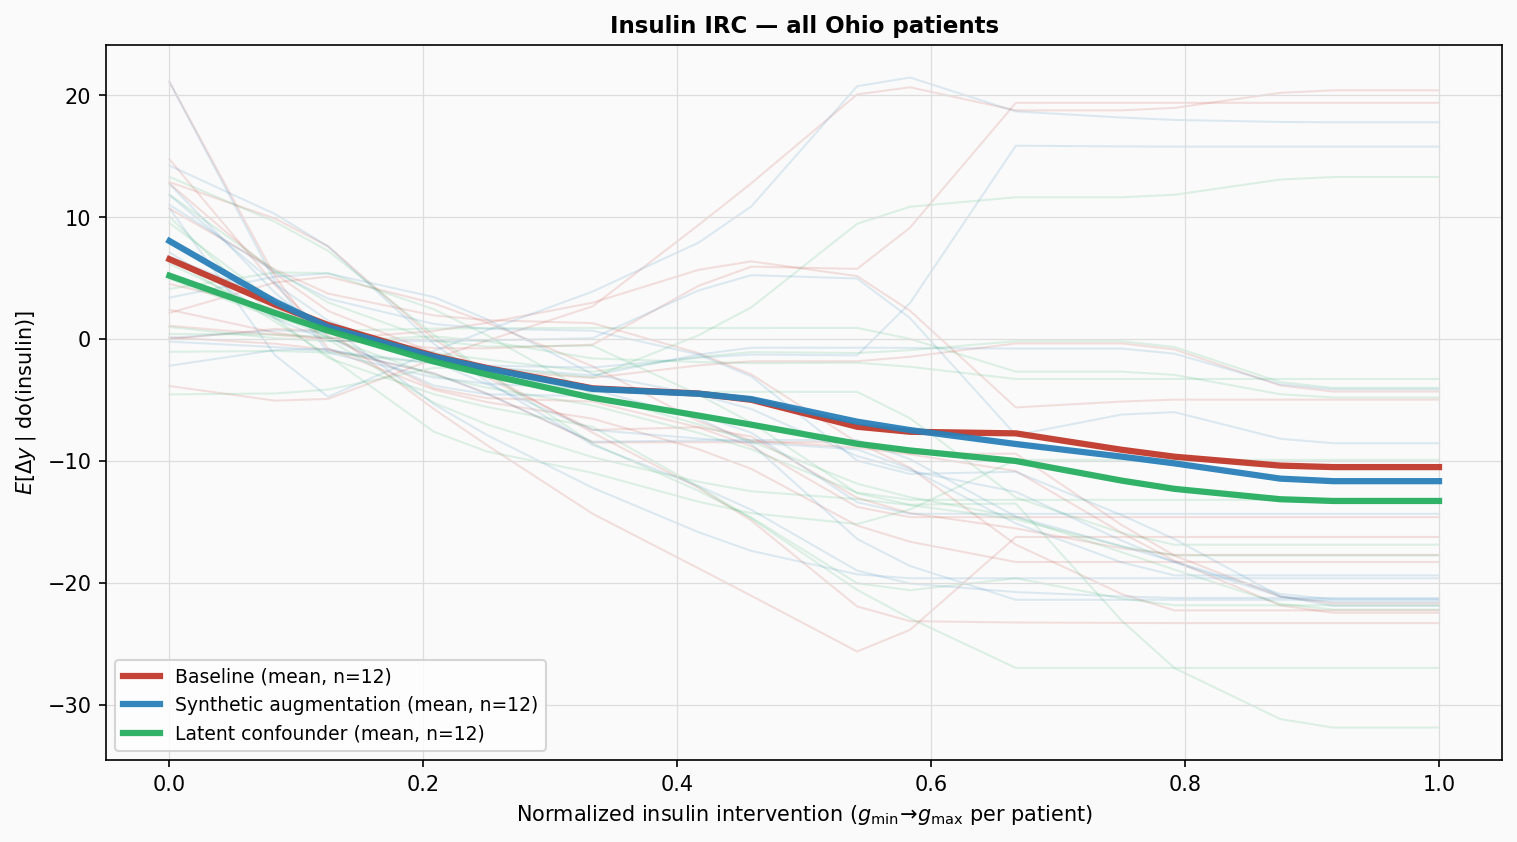
\includegraphics[width=\linewidth,height=0.44\textheight,keepaspectratio]{images/head_to_head_insulin_ircs.png}
\end{frame}

\end{document}
